\chapter{诊断算法解释性实验}

\section{实验设计}
我们通过在各大社交平台发布海报招募,如图\ref{fig:poster},以及使用问卷星的样本服务, 经过筛选之后,一共招募了100位左右的用户。
\begin{figure}[htb]
    \centering
    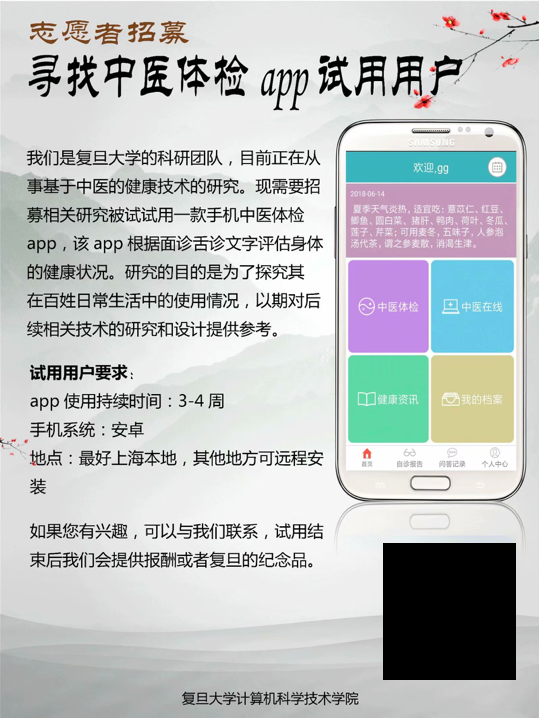
\includegraphics[height=8cm]{images/poster.png}
    \caption{招募海报}
    \label{fig:poster}
\end{figure}
\section{实验流程}

每个用户的实验流程如下:

1. 用户通过扫描二维码,或者通过我们给定的链接,进入问卷星调查问卷。

2. 完成调查问卷之后,自动进入云中医在线app。通过调用问卷星提供的企业用户接口, 同时把问卷星的问卷id通过ssojump传给云中医在线应用。通过ssojump中的问卷id, 完成自动登陆, 登陆的用户id为wjx-{问卷星id}, 透明类别为通过问卷星id哈希得到。

3. 在用户完成一次面诊之后,会在健康诊断页面下,看到一个跳转链接,可以选择填写用后问卷。

这样就把调查问卷信息,云中医应用使用日志和用后问卷数据关联起来了。


\section{实验数据获取}
每个用户在参与实验之后,我们可以得到调查问卷的数据,云中医的使用日志,已经用后问卷的数据。

调查问卷: 序号,提交答卷时间,所用时间,来源,来源详情,IP,个人信息	我相信中医养生,了解中医养生,平时注重养生,经常去看中医,希望自己的生活方式更健康,对学习相关中医养生知识感兴趣,认为中医面诊可以了解健康情况,认为中医舌诊可以了解健康情况,认为智能系统可以自动评估健康情况,随机顺序的中医知识问题

用后问卷: 序号,提交答卷时间,所用时间,来源,来源详情,IP,云中医的诊断结果,结果的信任程度,对结果的理解程度,是否愿意使用类似应用,随机顺序的中医知识问题

用户使用日志: 序号,用户名,设备信息,操作名,操作信息,日期 

个人信息包括性别,年龄段,受教育水平,职业,城市,健康状态等。

\subsubsection{关联规则}
对于同一个用户在一次实验过程中,若调查问卷的序号为ID, 则此次用户使用日志的用户名为wjx-ID, 用户问卷的来源详情为wjx-ID。 、
通过这个对应关系,我们就可以把三个表的信息,合并到一个表中, 最终得到特征如表\ref{tab:exp_data}所示。


\begin{table}[h]
    \centering
    \begin{tabular}{ll}
        \toprule
        字段 & 描述 \\ 
        \midrule
        序号 & 调查问卷序号 \\
        性别 & 男/女/未知 \\
        教育程度 & 本科以下/本科/本科以上 \\
        工作类型 & 计算机相关/计算机不相关 \\
        用户类型 & 透明/不透明 \\
        健康得分 & 云中医应用给出的分数 0-100 \\
        信任 & 对结果的信任程度 1-5 \\
        理解 & 对结果的理解程度 1-5 \\
        前健康知识得分 & 使用云中医之前的健康知识得分 \\
        后健康知识得分 & 使用云中医之后的健康知识得分 \\
        查看了哪些解释 & 使用过程中查看的解释类型 \\
        \bottomrule
    \end{tabular}
    \caption{实验数据汇总}
    \label{tab:exp_data}
\end{table}

表格 \ref{tab:exp_data}的字段说明如下:

工作类型: 根据调查问卷的数据,用户自由填写的职业类型有很多,为了便于分析,我们把 IT经理,IT软件设计, hr, it, 互联网, 技术研发, 技术研发人员, 技术经理, 电脑工程师, 研发, 科研, 程序员, 计算机, 软件工程师, 软件开发工程师, 通信, 通讯等归为it相关。

信任、理解: 这两个字段来自用后问卷调查表,取值范围为1-5的整数。

健康知识得分: 使用云中医应用前后的健康知识得分,使用的是用户回答正确中医知识的个数。

用户类型:透明类型的用户才能看到对结果以及术语的解释。

查看了哪些解释: 通过检索日志中关键字获取,包括面诊过程,舌诊过程,体质术语介绍,诊断报告的:面诊结果,舌诊结果,健康分数,体质,分数计算公式等。

\section{实验结果}

\subsection{用户是否愿意继续使用?}

\subsection{}

同时实验分析,我们可以得出,增加透明性可以提高用户对应中医知识的理解。

和看解释有关, 用 二元逻辑回归

把用户进行筛选,看了解释和没有看解释的

有解释的,看了没没看的(为什么看了,为什么没看), 

相关性分析,用于分析自变量

挑选相关性比较低的,放到后续的模型中 , 不加*,是很弱的 0.4-0.6比较强

了解中医养生,平时注重养生,了解中医养生
相信中医,了解中医

有没有看解释和it相关性不高

看了解释的影响:
独立样本t检验,差异性分析,没有显著差异

找最相似的不看解释的用户和看了解释的用户对比: 
对结果的信任和理解程度,两个样本没有显著差异



量化结果

定性实验

\section{结构性访谈}


